\documentclass[12pt]{scrartcl}

\setlength{\parindent}{0pt}
\setlength{\parskip}{.25cm}

\usepackage{graphicx}

\usepackage{xcolor}

\definecolor{darkred}{rgb}{0.5,0,0}
\definecolor{darkgreen}{rgb}{0,0.5,0}
\usepackage{hyperref}
\hypersetup{
  letterpaper,
  colorlinks,
  linkcolor=red,
  citecolor=darkgreen,
  menucolor=darkred,
  urlcolor=blue,
  pdfpagemode=none,
  pdftitle={CS1 Lab 1.0},
  pdfauthor={Christopher M. Bourke},
  pdfkeywords={}
}

\definecolor{MyDarkBlue}{rgb}{0,0.08,0.45}
\definecolor{MyDarkRed}{rgb}{0.45,0.08,0}
\definecolor{MyDarkGreen}{rgb}{0.08,0.45,0.08}

\definecolor{mintedBackground}{rgb}{0.95,0.95,0.95}
\definecolor{mintedInlineBackground}{rgb}{.90,.90,1}

%\usepackage{newfloat}
\usepackage[newfloat=true]{minted}
\setminted{mathescape,
               linenos,
               autogobble,
               frame=none,
               framesep=2mm,
               framerule=0.4pt,
               %label=foo,
               xleftmargin=2em,
               xrightmargin=0em,
               startinline=true,  %PHP only, allow it to omit the PHP Tags *** with this option, variables using dollar sign in comments are treated as latex math
               numbersep=10pt, %gap between line numbers and start of line
               style=default, %syntax highlighting style, default is "default"
               			    %gallery: http://help.farbox.com/pygments.html
			    	    %list available: pygmentize -L styles
               bgcolor=mintedBackground} %prevents breaking across pages
               
\setmintedinline{bgcolor={mintedBackground}}
\setminted[text]{bgcolor={mintedBackground},linenos=false,autogobble,xleftmargin=1em}
%\setminted[php]{bgcolor=mintedBackgroundPHP} %startinline=True}
\SetupFloatingEnvironment{listing}{name=Code Sample}
\SetupFloatingEnvironment{listing}{listname=List of Code Samples}

\title{CSCE 155 - Java}
\subtitle{Lab 1.0 - Introduction}
\author{~}
\date{~}

\begin{document}

\maketitle

\section*{Prior to Lab}

In each lab there may be pre-lab activities that you are \emph{required} to
complete prior to attending lab.  Failure to do so may mean that you will
not be given full credit for the lab.  For the first lab, there are no pre-lab
activities.

\section*{Peer Programming Pair-Up}

To encourage collaboration and a team environment, labs will be
structured in a \emph{pair programming} setup.  At the start of
each lab, you will be randomly paired up with another student 
(conflicts such as absences will be dealt with by the lab instructor).
One of you will be designated the \emph{driver} and the other
the \emph{navigator}.  

The navigator will be responsible for reading the instructions and
telling the driver what to do next.  The driver will be in charge of the
keyboard and workstation.  Both driver and navigator are responsible
for suggesting fixes and solutions together.  Neither the navigator
nor the driver is ``in charge.''  Beyond your immediate pairing, you
are encouraged to help and interact and with other pairs in the lab.

Each week you should alternate: if you were a driver last week, 
be a navigator next, etc.  Resolve any issues (you were both drivers
last week) within your pair.  Ask the lab instructor to resolve issues
only when you cannot come to a consensus.  

Because of the peer programming setup of labs, it is absolutely 
essential that you complete any pre-lab activities and familiarize
yourself with the handouts prior to coming to lab.  Failure to do
so will negatively impact your ability to collaborate and work with 
others which may mean that you will not be able to complete the
lab.  

\section{Lab Objectives \& Topics}
At the end of this lab you should be familiar with the following
\begin{itemize}
  \item The general lab environment \& CSE system including its policies and expectations
  \item Retrieving lab code from Github
  \item Modifying, compiling and executing your first Java 
    program using the Eclipse IDE (Integrated Development 
	Environment)
  \item Using CSE's webhandin and web grader
\end{itemize}

\section{Administrivia}

\subsection{Login \& Consent Form}

You will receive your login from the CSE System Administrators who will also 
give you an overview of the CSE system and its policies.  Be sure to login and 
change your temporary password.  Some departmental resources that you may
find useful:
\begin{itemize}
  \item CSE Website: \url{http://cse.unl.edu}
  \item UNL Computing Policy: \url{http://www.unl.edu/ucomm/compuse/}
   \item CSE Academic Integrity Policy: \url{http://cse.unl.edu/academic-integrity-policy}
   \item CSE System FAQ: \url{http://cse.unl.edu/faq}
   \item Account Management: \url{https://cse-apps.unl.edu/amu/}
   \item CSE Undergraduate Advising Page: \url{http://cse.unl.edu/advising}
   \item CSE Student Resource Center: \url{http://cse.unl.edu/src}
\end{itemize}

\subsection{Lab Introduction}

\begin{itemize}
  \item Lab instructors and TAs
  \item Office Hours
  \item Student Resource Center (Avery 12)
  \item Lab policies
\end{itemize}

\section{BYOD: Bring Your Own Device}

Though you can use the lab computers for this activity, you will
most likely want to use your own machine to do development independent
of the CSE labs.  To do this, you'll need to install a couple of
things.

\begin{enumerate}
  \item Go to Oracle's website and download and install the 
  Java Development Kit (JDK).  You may already have ``Java''
  installed but likely it is the \emph{Runtime Environment} (JRE)
  that allows you to run Java programs.  The Dev Kit allows you
  to \emph{develop} programs.  You should install the latest version;
  as of this writing the current version is 13 and is available at:
  \url{https://www.oracle.com/java/technologies/javase-jdk13-downloads.html}
  (alternatively, you can use openJDK instead if you wish: \url{https://openjdk.java.net/})
  \item Got to \url{https://www.eclipse.org/} and download/install
  the Eclipse IDE.  It is perfectly fine to use an alternative 
  IDE if you wish, but instructions for all labs will assume Eclipse.  
  \item Though not necessary for this lab, you should also sign
  up for a GitHub account: \url{https://github.com/}
\end{enumerate}

%\subsection{Basic Unix Commands}
%
%Much of your work will be done on the command line.  Take a moment to 
%familiarize yourself with the following basic commands.  A more comprehensive 
%tutorial on unix commands is available here: \url{http://www.math.utah.edu/lab/unix/unix-commands.html}.
%\begin{itemize}
%  \item Show the current working directory: \mintinline{text}{pwd}
%  \item Creating a new directory: \mintinline{text}{mkdir dirName}
%  \item Changing directories: \mintinline{text}{cd dir_name}
%  \item Moving up a directory: \mintinline{text}{cd ..}
%  \item Moving directly to your home directory: \mintinline{text}{cd ~}
%  \item Listing files in a directory: \mintinline{text}{ls}
%  \item Listing details of files in a directory: \mintinline{text}{ls -l}
%  \item Listing files in another directory: \mintinline{text}{ls dir_name}
%  \item Listing the contents of a (text) file: \mintinline{text}{more file_name}
%  \item Removing files (careful!):  \mintinline{text}{rm file_name}
%\end{itemize}
%
%\subsubsection*{Text Editors}
%
%Programming requires that you write code in a source file: a plain text file that 
%contains syntactically valid programming commands.  In general, any plain 
%text editor can facilitate this (MS Word is not a plain text editor).  The lab 
%instructor will demonstrate some of the following options: 
%\begin{itemize}
%  \item jpico
%  \item emacs
%  \item Notepad++ (a graphical editor launched from Windows)
%\end{itemize}
%
%\section{Activity A: Developing Java from the Command Line}
%
%\subsection{Checking Out Code From Github}
%
%Each lab will have some starter code and other \emph{artifacts} (data files, 
%scripts, etc.) that will be provided for to you.  However, the code is hosted
%on Github (\url{https://github.com}) and you must check it out.  You will not
%need to know the details of using git nor be a registered Github user to 
%get access to the code necessary for your labs or assignments.  However, 
%you are \emph{highly encouraged} to learn this essential tool.  You may find
%it very useful to keep track of your own code and to share code if you work
%in pairs or groups.  
%
%To check out the code for this lab, do the following.
%\begin{enumerate}
%  \item If you haven't already, connect to the CSE server using PuTTY as follows:
%  \begin{enumerate}
%    \item Open PuTTY (this is a Secure Shell Client, SSH)
%    \item Enter the address \mintinline{text}{cse.unl.edu}
%    \item Click ``Open''
%    \item Login using your CSE credentials (you may be prompted to change your password the first time).
%  \end{enumerate}
%  \item In your home directory, create a new directory for all your labs:\\  
%  \mintinline{text}{mkdir labs}  
%  \item Verify that this worked by listing the contents of your directory by
%  typing \mintinline{text}{ls}.  You should see your \mintinline{text}{labs} directory.
%   \item Go to this directory by changing your directory:\\
%  \mintinline{text}{cd labs}
%  \item ``Clone'' this lab's code by using the following command:\\
%  \mintinline{text}{git clone https://github.com/cbourke/CSCE155-Java-Lab01}
%  \item A new directory, \mintinline{text}{CSCE155-Java-Lab01} should be created, 
%  go to this directory by typing \mintinline{text}{cd CSCE155-Java-Lab01/src}.
%  \item List the contents of this directory by typing \mintinline{text}{ls}.  If
%  everything worked, there should be a \mintinline{text}{Hello.java} file in your
%  directory.
%\end{enumerate}
%
%\subsection{Your First Program: Hello World!}
%
%As this is an introductory course, most of the Java programs you will write in 
%this course will execute and require interaction from the command line 
%rather than a more user-friendly graphical interface.  
%
%The code you cloned contains a basic ``Hello World'' program that, when
%compiled and run will simply print the message ``Hello World'' and exit.
%
%To compile and run this program, do the following.
%\begin{enumerate}
%  \item Type \mintinline{text}{javac Hello.java}, this \emph{compiles} the source code
%  	into a \emph{class file} named \mintinline{text}{Hello.class}.\footnote{The
%	class file contains Java Byte Code that can be interpreted and executed
%	in a Java Virtual Machine (JVM)}  Use 
%	\mintinline{text}{ls} to verify that the new file has been created. 
%  \item Run your program by typing the following: \mintinline{text}{java Hello}
%\end{enumerate}
%
%Note: \mintinline{text}{javac} is the Java \textbf{c}ompiler while the 
%\mintinline{text}{java} command launches the Java Virtual Machine 
%from the command line.
%
%Let's now modify the program. 
%
%\begin{enumerate}
%  \item Open the \mintinline{text}{Hello.java} source file in the text editor of
%  	your choice (Notepad++ is recommended for beginners).
%  	Your program should look something like the following:
%
%\begin{minted}{java}
%/**
%  Author: Chris Bourke
%  Date: xx/xx/20xx
%  Hello World in Java 
%*/ 
%public class Hello {
%  
%  public static void main(String args[]) {
%    System.out.println("Hello World!");
%  }
%}
%\end{minted}
%  \item Modify the file by changing the author to you and your partner and change
%  	the date.
%  \item Change the message that is produced by the program (line 9) to instead
%  	print you and your partner's names.
%  \item Save and exit your editor and repeat the process to compile and run
%  	your program and verify that your changes have taken effect.
%\end{enumerate}

\section{Activity: Creating a New Project}

\subsection{Using Eclipse}

Eclipse is an industry-standard IDE for Java development.  
There are several other popular and emerging IDEs available 
and you are welcome (and encouraged) to try them out and use 
them.  For this course, we will primarily focus on Eclipse.

\begin{enumerate}
  \item From Windows, start Java Eclipse
  \item Choosing a ``Workspace'':
  \begin{itemize}
    \item If you are using a lab computer, type the following in the 
    text box: \mintinline{text}{Z:\Workspace} (the Z: drive is your 
    personal file storage on CSE)
	\item If you are using a personal computer, choose a workspace 
	directory/folder where you want all of your future projects to 
	exist.
  \end{itemize}
  \item Close the Welcome screen, and create a new project.  
    Select:  File $\rightarrow$ New $\rightarrow$ Project
  \item Select ``Java Project'' when prompted by the New Project Wizard; click Next
  \item Enter a name for your project (Lab01); click Finish
  \item Open the Lab01 folder in the Package Explorer View and find the \mintinline{text}{src} folder
  \item Right-click on the \mintinline{text}{src} folder and select ``New Class'' and name it \mintinline{text}{Hello}.
  \item This should open a new source code editor.  Make your program
  look like the following and save it.
\begin{minted}{java}
public class Hello {

  public static void main(String args[]) {
    System.out.println("Hello World!");
  }

}
\end{minted}
  \item Run your program by clicking the ``play'' button in the tool bar
\end{enumerate}

Congratulations on your first program!

\section{Checking Out Code From Github}

Each lab will have some starter code and other \emph{artifacts} (data files, 
scripts, etc.) that will be provided for to you.  However, the code is hosted
on Github (\url{https://github.com}) and you must check it out.  You will not
need to know the details of using git nor be a registered Github user to 
get access to the code necessary for your labs or assignments.  However, 
you are \emph{highly encouraged} to learn this essential tool.  You may find
it very useful to keep track of your own code and to share code if you work
in pairs or groups.  

\begin{enumerate}
  \item First we need a Git \emph{perspective} (a context in the Eclipse 
    User Interface that will allow us to work with Git).  To open the 
    Git perspective, click on the ``Open Perspective'' tab in the upper right:
	\begin{center}
	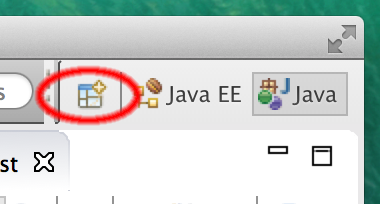
\includegraphics[scale=0.50]{eclipseOpenPerspectiveMarkUp}
	\end{center}
	Select ``Git'' from the menu and click OK
  \item Click the ``Clone a Git repository'' in the Git Repositories navigation menu:
  	\begin{center}
	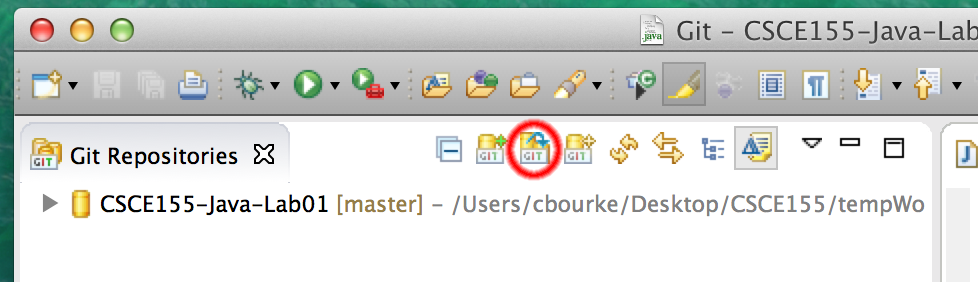
\includegraphics[scale=0.50]{eclipseGitRepoMarkUp}
	\end{center}
  \item Copy/past or type into the URI field, the URL: \\
  	\url{https://github.com/cbourke/CSCE155-Java-Lab01}
  	\begin{center}
	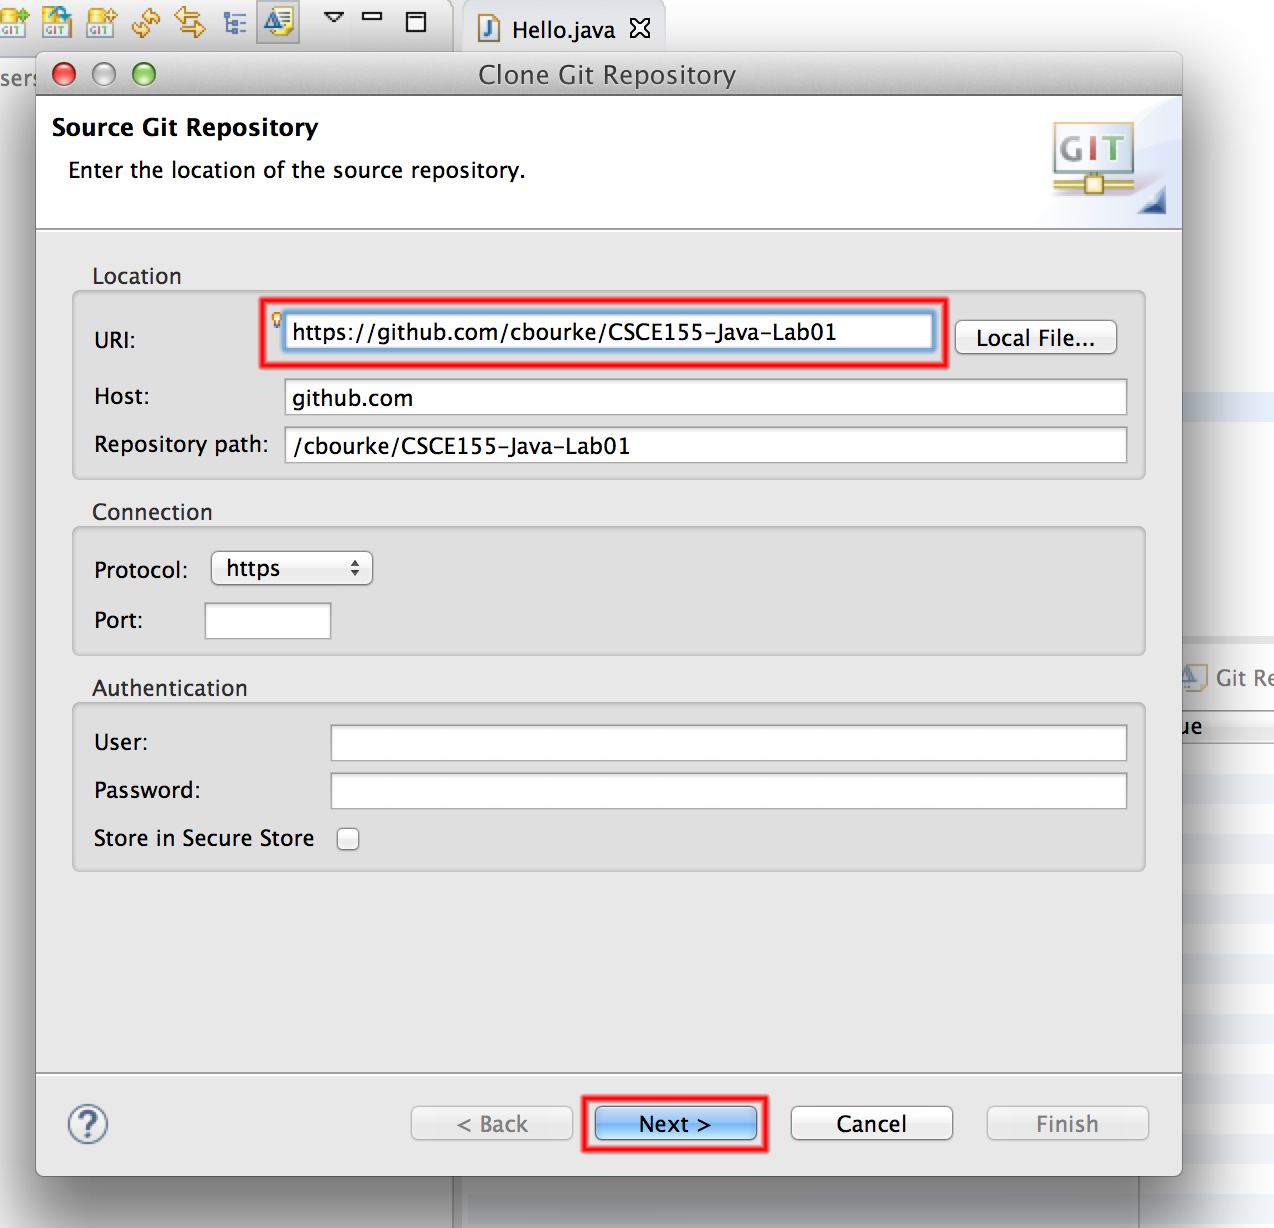
\includegraphics[scale=0.35]{eclipseCloneDialogAMarkUp}
	\end{center}
  \item Click ``Next''; once Eclipse has grabbed the project, the ``master'' branch should
  	be selected (checkbox); click ``Next'' again.
  	\begin{center}
	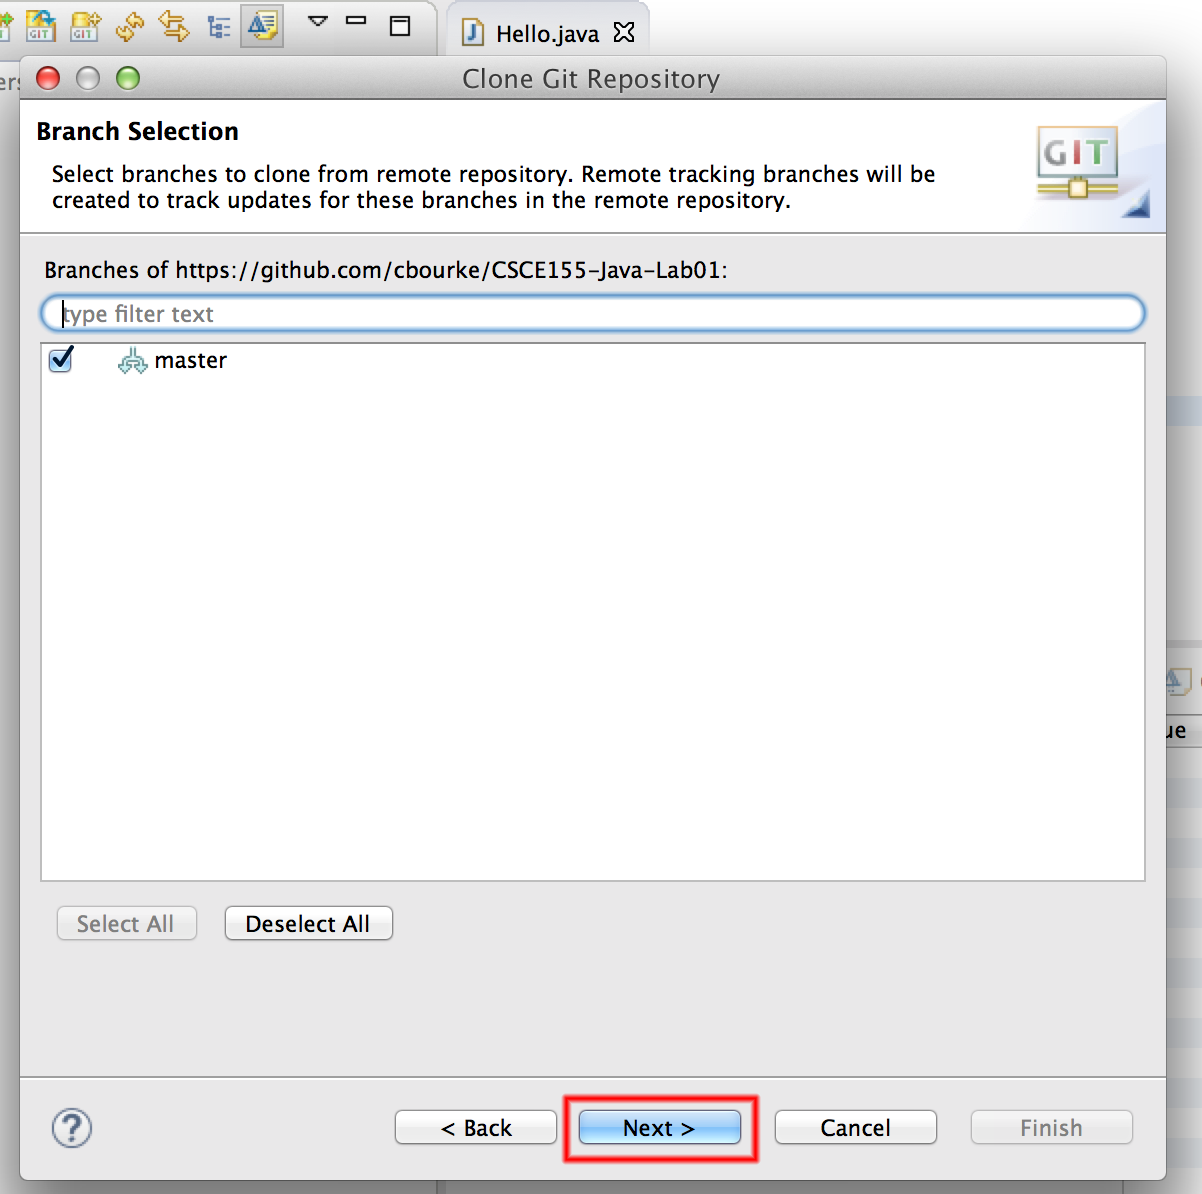
\includegraphics[scale=0.35]{eclipseCloneDialogBMarkUp}
	\end{center}
  \item Select the directory where you want your project to be saved.  Caution: the default
  	option may not correspond to your default workspace.  You may want to change
	it to your workspace, but the choice is yours.  Also mark the ``Import all existing 
	projects after clone finishes'' checkbox option or you will need
  	to manually import the cloned project into Eclipse.
  	\begin{center}
	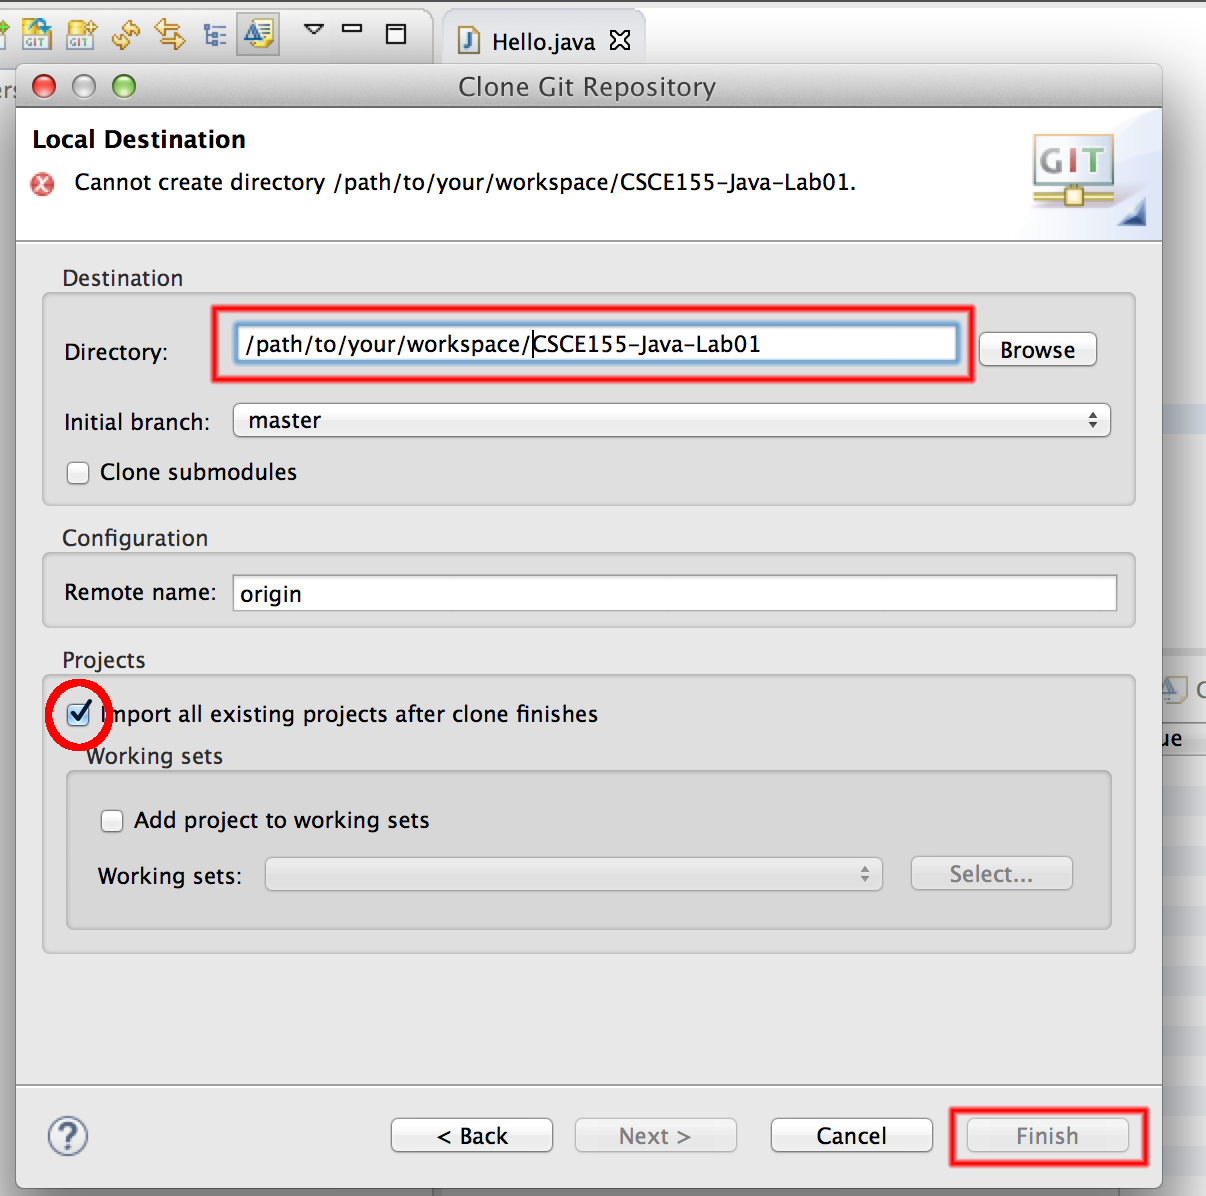
\includegraphics[scale=0.35]{eclipseCloneDialogCMarkUp}
	\end{center}
  \item Switch back to your Java or JavaEE perspective and you can see your cloned 
  	project.  
  \item Run the \mintinline{java}{Hello.java} program in this 
  project to verify everything works.
\end{enumerate}

\subsection{Modify the Program}

\begin{enumerate}
  \item Modify the \mintinline{java}{Hello.java} program by changing the 
  author to you (and your partner) and change the date.
  \item Change the message that is printed by the program to instead
  	print you (and your partner's) name(s).
\end{enumerate}


\section{Handing In \& Grading}

Many of your assignments will include a programming portion that will 
require you to hand in \emph{soft-copy} source files for graders to compile 
and evaluate.  To do this, you will use a web-based handin program.  
After handing your file(s) in, you can then grade them by using the
web grader.  To demonstrate, do the following.

\begin{enumerate}
  \item Open a browser to \url{https://cse-apps.unl.edu/handin}
  \item Login with your CSE credentials
  \item Click on this course/lab 01 and handin the \mintinline{text}{Hello.java} file.  You can
  either click the large ``handin'' area and select the file or you can drag-drop
  the file.  You will be able to re-handin the same file as many times as you want up until
  the due date.
  \item Now that the file has been handed in, you can ``grade'' 
  yourself by using the webgrader; open a new tab/window and point 
  your browser to one of the following depending on which course 
  you are in:
  \begin{itemize}
    \item \url{https://cse.unl.edu/~cse155a/grade}
    \item \url{https://cse.unl.edu/~cse155e/grade}
    \item \url{https://cse.unl.edu/~cse155h/grade}
  \end{itemize}
  \item Fill the form with your CSE login and password, select the 
  appropriate assignment and click ``Grade''
  \item For future assignments and labs, you can compare the results of 
  	your program with the ``Expected Results''.  If there are problems or errors with
	your program(s), you should fix/debug them and repeat the handin/grading process.
	You can do this as many times as you like up until the due date.  Some programs 
	and assignments will run test cases and may provide expected output alongside 
	your output.  Others may have more sophisticated test cases and actually provide 
	you a percentage of test cases passed.  It is your responsibility to read, 
	understand and \emph{address} all of the errors and/or warnings that the grader produces.
\end{enumerate}

\end{document}
